\newpage
\section{Mô hình hồi quy tuyến tính đơn biến}
\subsection{Xây dựng mô hình}
\subsubsection{Phương pháp xây dựng}
\paragraph{}{Ta sử dụng \textbf{phương pháp bình phương tối thiểu} (Ordinary Least Squares - OLS) (xem \ref{label:simple-linear}). Phương pháp này tìm cách tối thiểu hóa tổng bình phương của các sai số giữa giá trị thực tế và giá trị dự đoán. Điều này giúp MSE của mô hình là thấp nhất.}
\subsubsection{Công thức hồi quy}
\paragraph{}{Thông qua ma trận tương quan (hình \ref{fig:corr-matrix-2}), ta thấy đặc trưng \texttt{Model} có sự tương quan lớn với \texttt{Price}. Qua thực nghiệm, \texttt{Model} là đặc trưng tốt nhất để xây dựng mô hình hồi quy tuyến tính đơn.}

\begin{center}
\large $Price = 52041.63 + 27427303.62 * Model$
\end{center}

Trong đó:
\begin{itemize}
    \item $Price$: Giá xe được dự đoán bởi mô hình
    \item $Model$: Giá trị của đặc trưng \texttt{Model} sau các quá trình xử lí dữ liệu. \footnote{Sau các quá trình tiền xử lý, mã hóa và chuẩn hóa dữ liệu. Trong đó đóng góp tích cực nhất là quá trình mã hóa đặc trưng \texttt{Model} bằng các giá trị trung vị của giá xe tương ứng.}
\end{itemize}

\subsection{Đánh giá mô hình}

\begin{figure}[H]
    \centering
    \begin{subfigure}[b]{0.48\textwidth}
        \centering
        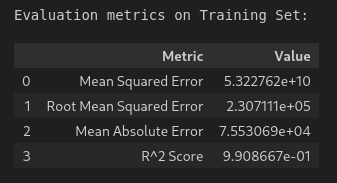
\includegraphics[width=\linewidth]{img/simple-linear-train.png}
        \caption{Đánh giá trên tập huấn luyện}
        \label{fig:simple-linear-train}
    \end{subfigure}
    \hfill
    \begin{subfigure}[b]{0.48\textwidth}
        \centering
        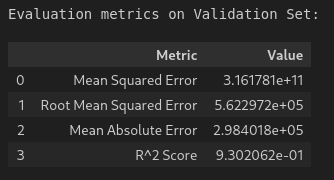
\includegraphics[width=\linewidth]{img/simple-linear-valid.png}
        \caption{Đánh giá trên tập kiểm chứng}
        \label{fig:simple-linear-valid}
    \end{subfigure}
    \caption{So sánh đánh giá mô hình trên tập huấn luyện và kiểm chứng} 
    \label{fig:simple-linear-eval}
\end{figure}

\paragraph{}{Trên tập huấn luyện, mô hình đạt MSE là $5.322762 * 10^{10}$ và R² là $0.9908$, cho thấy mô hình rất khớp với dữ liệu đã thấy. Tuy nhiên, trên tập kiểm chứng, MSE tăng lên đáng kể thành $3.161781 * 10^{11}$ và R² giảm xuống còn 0.9302.}

\paragraph{}{Mặc dù R² trên tập kiểm chứng vẫn khá cao, sự gia tăng đáng kể của các chỉ số lỗi (MSE tăng gấp 6 lần) cho thấy dấu hiệu của hiện tượng overfitting. Mô hình đã học thuộc một số đặc điểm nhiễu của tập huấn luyện và khả năng tổng quát hóa trên dữ liệu mới bị hạn chế hơn. Điều này cũng có thể quan sát thấy trong hình \ref{fig:simple-linear}, nơi các điểm dữ liệu kiểm chứng phân tán rộng hơn quanh đường dự đoán so với tập huấn luyện. Tuy nhiên, điều này có thể  chấp nhận được vì đây chỉ là mô hình hồi quy tuyến tính đơn.}

\begin{figure}[H]
    \centering
    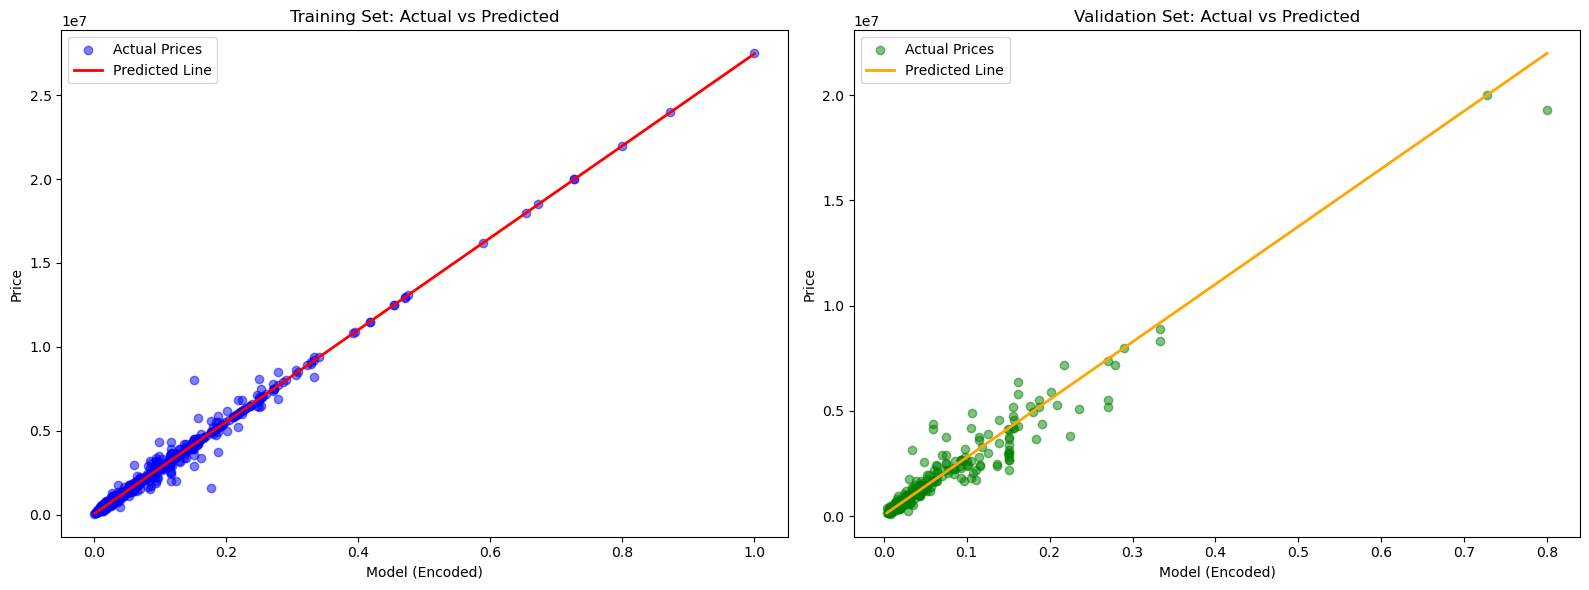
\includegraphics[width=1\linewidth]{img/simple-linear.png}
    \caption{Đường thẳng hồi quy dự đoán so với thực tế, trên tập huấn luyện và kiểm chứng}
    \label{fig:simple-linear}
\end{figure}

\pagebreak